\documentclass[tikz]{standalone}
\usepackage{tikz}
\usetikzlibrary{positioning, graphs}
\usetikzlibrary{graphs.standard}
\begin{document}
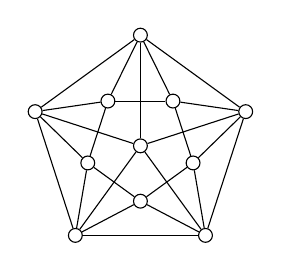
\begin{tikzpicture}
\begin{scope}
		[every node/.style={draw, circle,inner sep = 0em, minimum size = 0.5em}]
		\graph[clockwise, radius = 4em, empty nodes, phase = 18]{subgraph C_n[n = 5, name = A]};
		\graph[clockwise, radius = 2em, empty nodes, phase = -18] {subgraph C_n [n = 5, name = B]};
		
		\node (a) at (0,0) {};		
		
		\foreach \i [evaluate={\j=int(mod(\i+3,5)+1);}] in {1,...,5}{
		\draw (A \i) -- (B \i);
		\draw (A \i) -- (B \j);
		\draw (A \i) -- (a);
		}
\end{scope}
\end{tikzpicture}
\end{document}